% !TEX root = ../thesis.tex

\chapter{Anhang}
\label{anhang}

\begin{figure}[H]
    \centering
    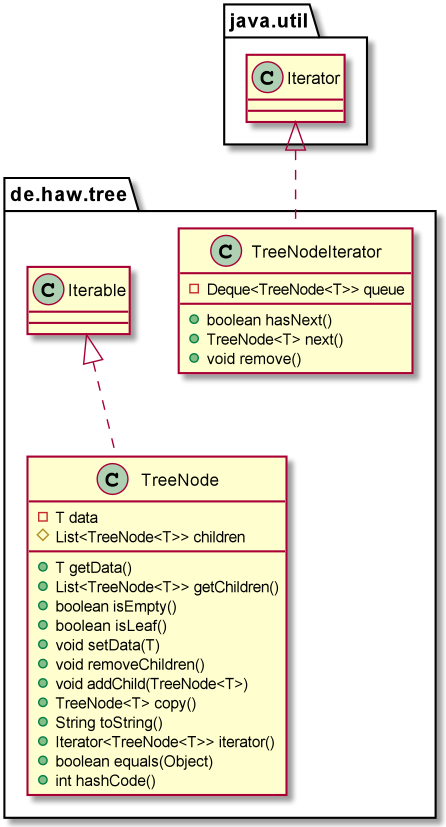
\includegraphics[width=6cm]{../images/tree.png}
    \caption{Baumstruktur}
    \label{tree}
\end{figure}

\begin{figure}[H]
    \centering
    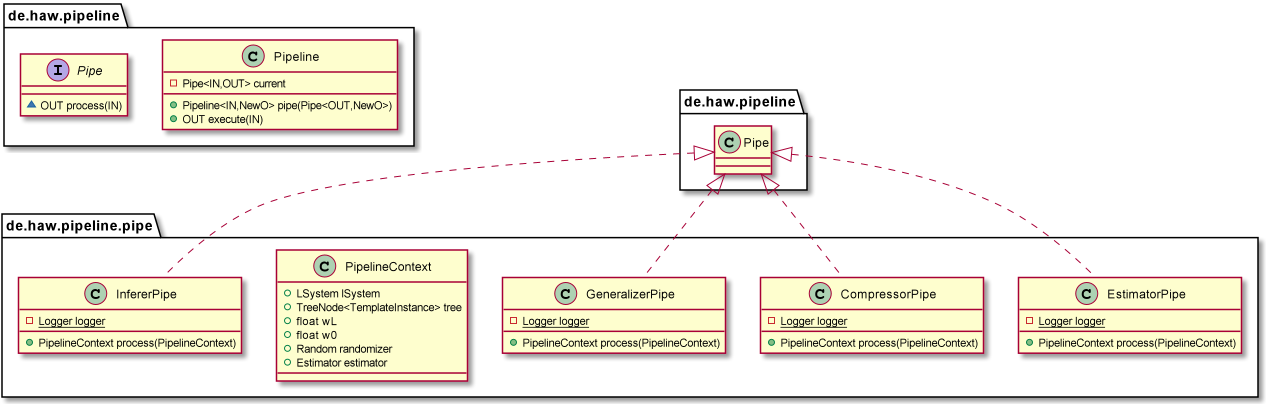
\includegraphics[width=22cm,angle=90]{../images/pipeline.png}
    \caption{Pipeline}
    \label{pipeline}
\end{figure}

\begin{figure}[H]
    \centering
    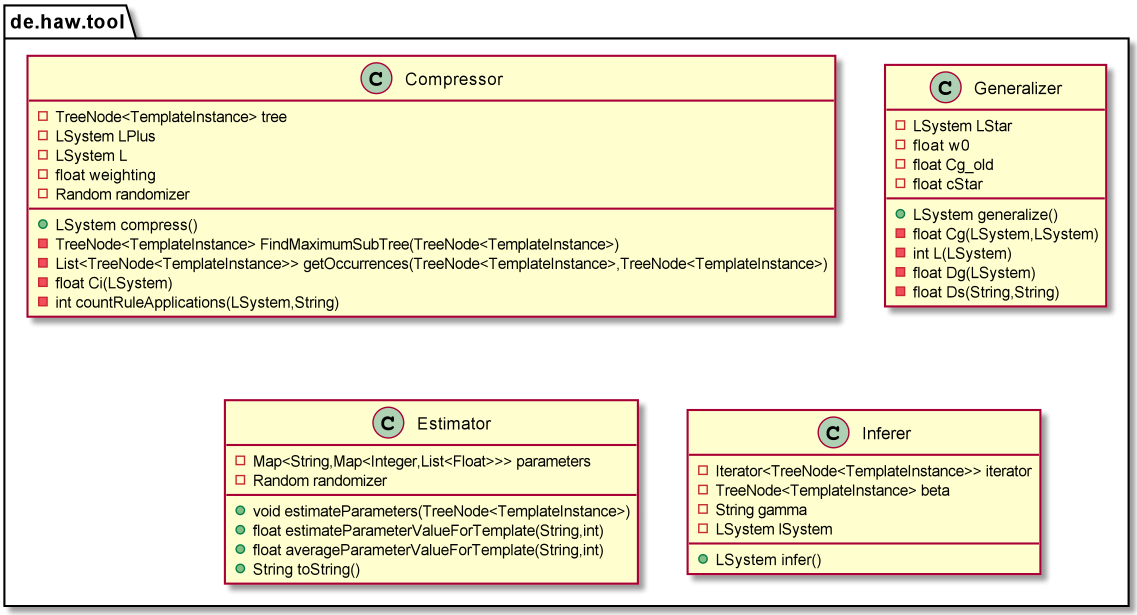
\includegraphics[width=14.8cm]{../images/tool.png}
    \caption{Subsysteme der Generierungs-Pipeline}
    \label{tool}
\end{figure}

\begin{figure}[H]
    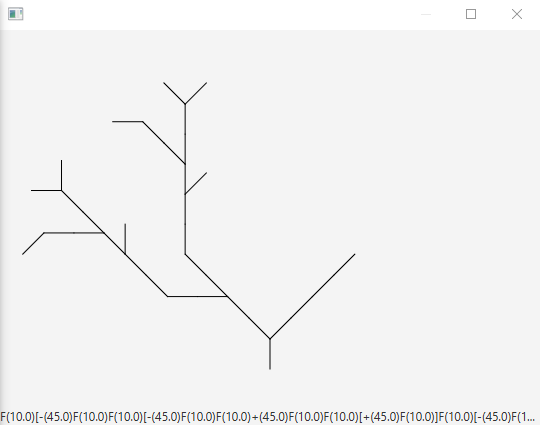
\includegraphics[width=6cm]{../images/example_1.png}
    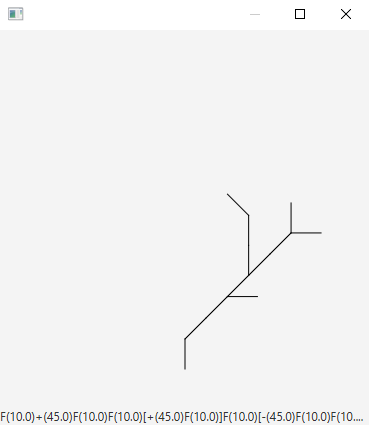
\includegraphics[width=6cm]{../images/example_2.png}
    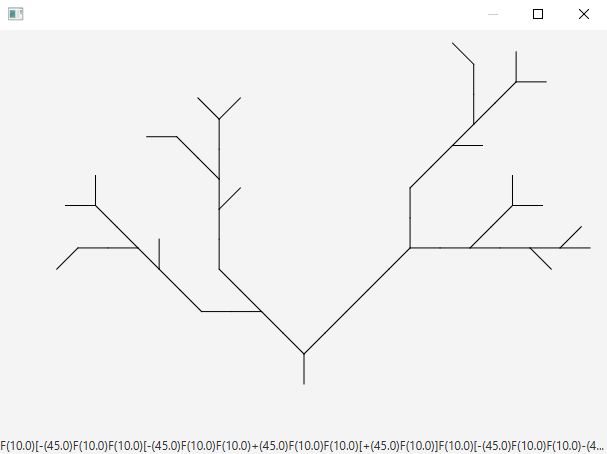
\includegraphics[width=6cm]{../images/example_3.png}
    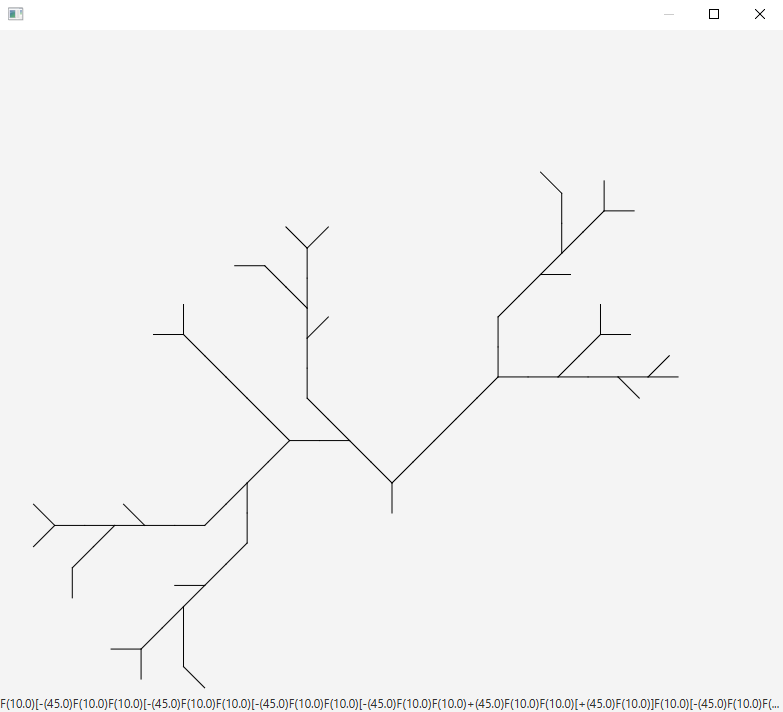
\includegraphics[width=6cm]{../images/example_4.png}
    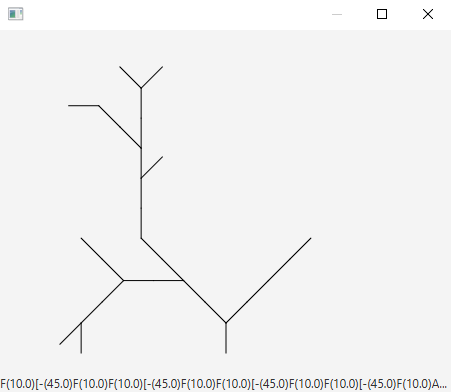
\includegraphics[width=6cm]{../images/example_5.png}
    \caption{Generierte Verzweigungsstrukturen}
    \label{resulting_structures}
\end{figure}

\newpage

\begin{lstlisting}[
    label=infer,
    basicstyle=\footnotesize,
    breaklines = true,
    commentstyle=\color{comment},
    keywordstyle=\color{keyword},
    language=Java,
    numberstyle=\color{gray},
    numbers = left,
    caption=Inferrierungsalgorithmus der Inferer Klasse,
    frame=tB,
    postbreak=\mbox{\textcolor{gray}{\ArrowBoldDownRight}\space}
]
/**
 * Return a L-System inferred from the given tree structure
 * @return Inferred L-System
 */
public LSystem infer() {
    var done = false;
    while (!done) {
        // delta = word of beta
        var delta = (beta == null || beta.isEmpty()) ? "" : beta.getData().getTemplate().getWord();
        // For all variables in delta
        var variableMatches = Pattern.compile("[A-EG-Z]")
                .matcher(delta)
                .results()
                .collect(Collectors.toList());
        for (var v : variableMatches) {
            var index = delta.indexOf(v.group(0));
            // Add new module not present in the alphabet
            String zeta = lSystem.addModuleNotPresentInAlphabet();
            // Replace variable with new module not present in alphabet
            delta = delta.substring(0, index) + zeta + delta.substring(index + 1);
        }

        // R <- { gamma -> delta }
        lSystem.addProductionRule(new ProductionRule(gamma, delta));

        // Find an eta that is in the alphabet but not part of the LHS of any production rule
        var modules = lSystem.getAlphabet();
        for (var eta : modules) {
            if (eta.equals("F")) continue;
            if (eta.equals("S")) continue;
            var lhs = lSystem.getProductionRules().stream()
                    .map(ProductionRule::getLhs)
                    .filter(x -> x.equals(eta))
                    .findFirst()
                    .orElse(null);

            if (lhs == null) {
                gamma = eta;
                break;
            }

            // There is no symbol in the alphabet not being part of a lhs of a production rule?
            if (modules.indexOf(eta) == modules.size() - 1) done = true;
        }
        beta = iterator.next();
    }
    return lSystem;
}
\end{lstlisting}

\begin{lstlisting}[
    label=compress,
    basicstyle=\footnotesize,
    breaklines = true,
    commentstyle=\color{comment},
    keywordstyle=\color{keyword},
    language=Java,
    numberstyle=\color{gray},
    numbers = left,
    caption=Komprimierungsalgorithmus der Compressor Klasse,
    frame=tB,
    postbreak=\mbox{\textcolor{gray}{\ArrowBoldDownRight}\space}
]
/**
 * Return a compressed L-System by finding maximum sub-trees
 * and replacing them
 * @return Compressed L-System
 */
public LSystem compress() {
    // T' <- T
    var subtree = FindMaximumSubTree(tree);
    while (subtree != null && !subtree.isEmpty()) {
        // Get extended string representation from (repetitive) sub tree
        var subTreeDerivation = new Inferer(subtree).infer().derive();
        // Data to be set in the tree to replace old node structure representing the subtree
        Template template = new Template(subTreeDerivation);
        // Estimate parameters for new template instance derivation
        var estimator = new Estimator(randomizer);
        var occurrences = getOccurrences(subtree, tree);
        // Average parameter
        for (var o : occurrences) {
            estimator.estimateParameters(o);
        }
        // Replace occurrences of the sub tree
        for (var o : occurrences) {
            var derivationInstance = new TemplateInstance(template);

            int scalingSum = 0, rotationSum = 0, branchingAngleSum = 0;
            int counter = 0;
            for (var node : o) {
                if (node.isEmpty()) continue;
                counter++;
                scalingSum += estimator.averageParameterValueForTemplate("Scaling", node.getData().getTemplate().getId());
                rotationSum += estimator.averageParameterValueForTemplate("Rotation", node.getData().getTemplate().getId());
                branchingAngleSum += estimator.averageParameterValueForTemplate("Branching angle", node.getData().getTemplate().getId());
            }

            derivationInstance.setParameter("Scaling", (float) (scalingSum / counter));
            derivationInstance.setParameter("Rotation", (float) (rotationSum / counter));
            derivationInstance.setParameter("Branching angle", (float) (branchingAngleSum / counter));

            o.setData(derivationInstance);
            o.removeChildren();
        }
        L = new Inferer(tree).infer().minimize();
        if (Ci(L) >= Ci(LPlus)) {
            break;
        }
        // T <- T'
        subtree = FindMaximumSubTree(tree);
        // L+ <- L
        LPlus = L;
    }

    return LPlus.clean();
}
\end{lstlisting}

\newpage

\begin{lstlisting}[
    label=generalize,
    basicstyle=\footnotesize,
    breaklines = true,
    commentstyle=\color{comment},
    keywordstyle=\color{keyword},
    language=Java,
    numberstyle=\color{gray},
    numbers = left,
    caption=Generalisierungsalgorithmus der Generalizer Klasse,
    frame=tB,
    postbreak=\mbox{\textcolor{gray}{\ArrowBoldDownRight}\space}
]
/**
 * Generalize a L-System by adding non-deterministic rules
 * @return Generalized L-System
 */
public LSystem generalize() {
    do {
        // Exclude S -> A from set combinations
        var productionRulesWithoutS = new ArrayList<>(LStar.getProductionRules());
        if (productionRulesWithoutS.remove(0) == null)
            throw new RuntimeException("No rule S -> A found");
        // Generate all possible merging rule pairs P ∈ L*
        var combinations = Sets.combinations(new HashSet<>(productionRulesWithoutS), 2);
        var minimalCosts = Float.MAX_VALUE;
        LSystem minimalLSystem = null;
        // Find a pair p_i with the minimal Cg(L* + {p_i}, L*)
        for (var c : combinations) {
            var LStarMerged = LStar.merge(c);
            float costs = Cg(LStarMerged, LStar);
            if (costs < minimalCosts) {
                minimalCosts = costs;
                minimalLSystem = LStarMerged;
            }
        }
        if (minimalCosts >= 0) break;
        cStar = minimalCosts - Cg_old;
        Cg_old = minimalCosts;
        LStar = minimalLSystem;
    } while (cStar <= 0);

    return LStar;
}
\end{lstlisting}

\newpage

\begin{lstlisting}[
    label=estimate,
    basicstyle=\footnotesize,
    breaklines = true,
    commentstyle=\color{comment},
    keywordstyle=\color{keyword},
    language=Java,
    numberstyle=\color{gray},
    numbers = left,
    caption=Verteilungsalgorithmus der Estimator Klasse,
    frame=tB,
    postbreak=\mbox{\textcolor{gray}{\ArrowBoldDownRight}\space}
]
...
/**
 * Create transformation parameter distribution of a given tree
 * @param tree Tree the parameters are distributed from
 */
public void estimateParameters(TreeNode<TemplateInstance> tree) {
    // Determine different parameters
    tree.getData().getParameters().forEach((key, value) -> parameters.putIfAbsent(key, new HashMap<>()));
    // Iterate tree and extract parameters
    for (var node : tree) {
        if (node == null || node.isEmpty()) continue;
        var templateID = node.getData().getTemplate().getId();
        for (var p : node.getData().getParameters().entrySet()) {
            var parameterEntry = parameters.get(p.getKey());
            var templateEntry = parameterEntry.get(templateID);
            if (templateEntry == null) {
                var valueList = new ArrayList<Float>();
                valueList.add(p.getValue().floatValue());
                parameterEntry.put(templateID, valueList);
            } else {
                templateEntry.add(p.getValue().floatValue());
            }
        }
    }
}
...
\end{lstlisting}

\begin{figure}[H]
    \centering
    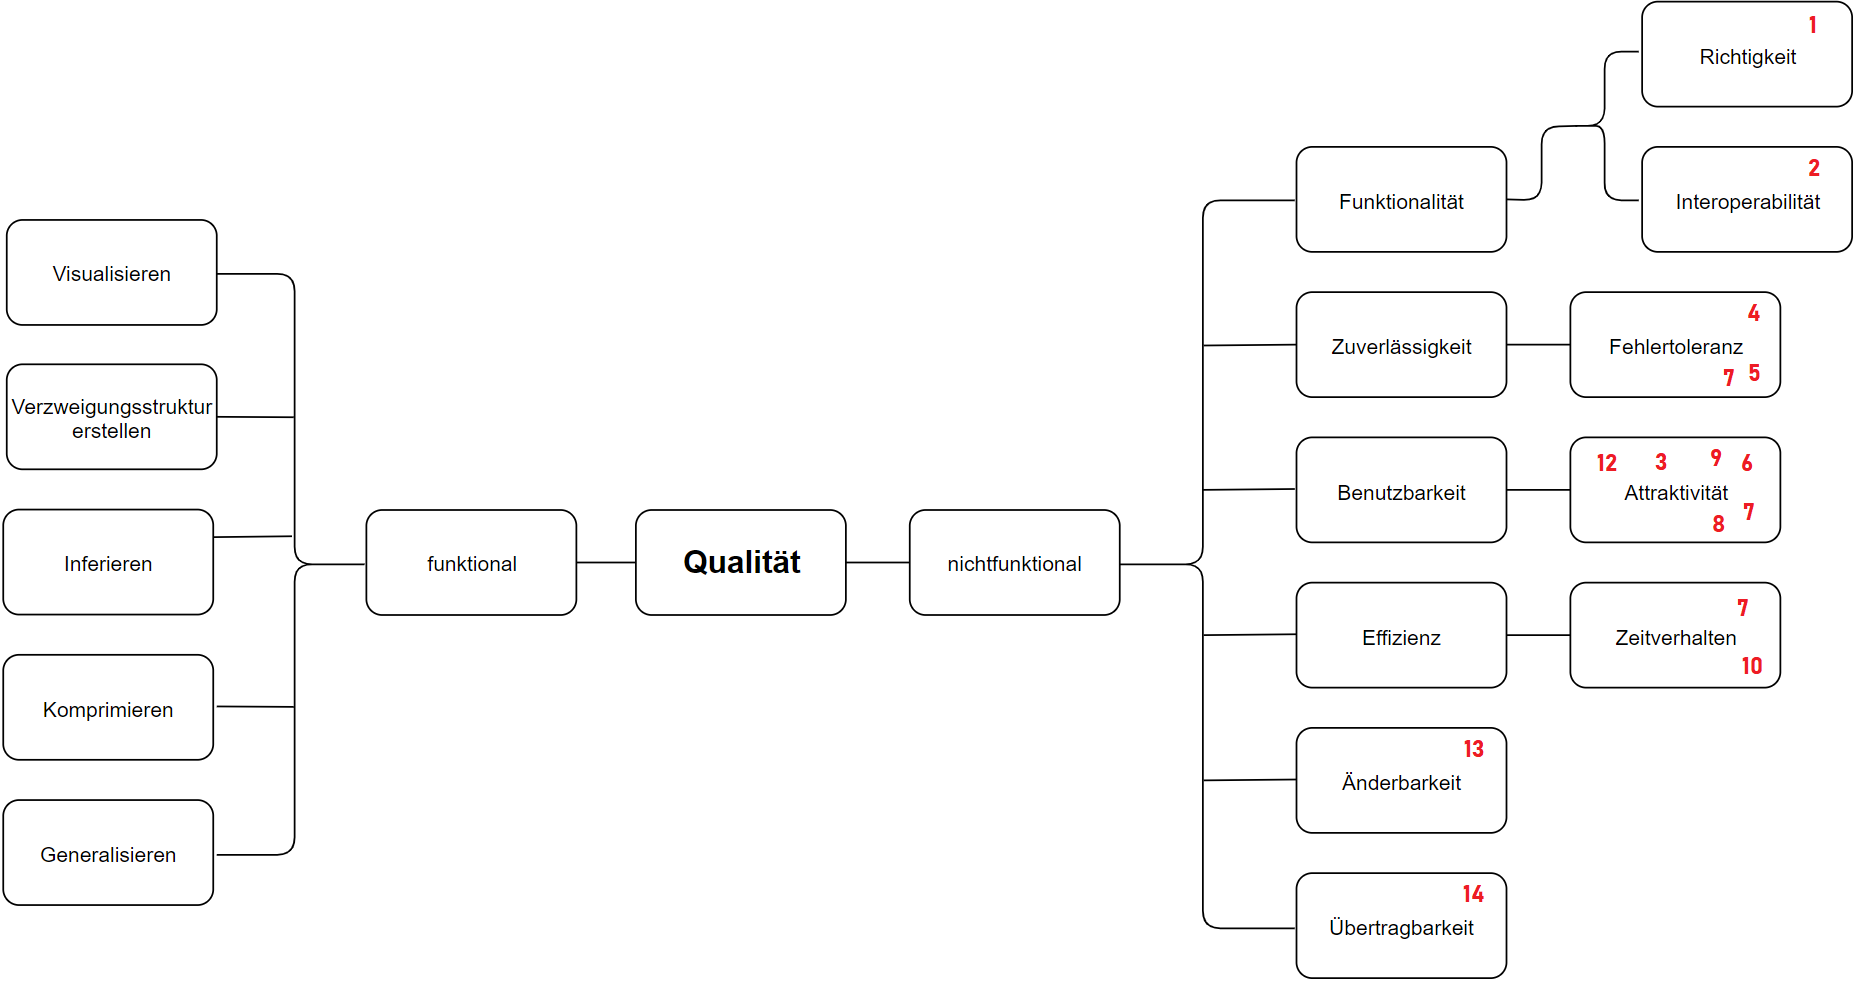
\includegraphics[width=18cm,angle=90]{../images/baum_nummern.png}
    \caption{Qualitätsbaum}
    \label{baum}
\end{figure}